%!TEX root = ../username.tex
\chapter{Physics of Sound Waves}\label{chapter:theory}

\section{Mathematical Background}\label{section:waveforms}
According to Joseph Fourier, the creator of the Fourier Transform, any periodic signal or sound can be reduced into their individual sine waves, or other waveform types \cite{Broughton_Bryan_2008}. There are five basic periodic waveform types: a sine wave, square wave, sawtooth wave, triangle wave, and pulse wave \cite{Winer_2018}. Each of these waveforms, except for the pulse wave, are sinusoidal waveforms which repeat in a pattern of motion known as a cycle. From this, we calculate the \textit{period} to be the time length between a cycle. The pulse wave is a special type of waveform, with its own individual characteristics, different from the other four periodic waveform types. As a non-sinusoidal waveform, or a wave which does not oscillate similar to the repetitive oscillation of a sine wave, it may assist in the creation of square waves, a waveform which is periodic and sinusoidal in nature. However, for the purposes of this work, the pulse wave will not be discussed within the scope of this project, due to its nature as a non-periodic and non-sinusoidal waveform, two waveform types which are not included in this synthesizer. The remaining four periodic waveforms each also have an individual sound and characteristics, and thus will be used for different types of sound synthesis and applications.

In its most basic form, there are three general types of waves \cite{Halliday_Resnick_Walker_2005}.

\begin{enumerate}
	\item Mechanical waves.
	\item Electromagnetic waves.
	\item Matter waves.
\end{enumerate}

Mechanical waves are the most familiar to many, due to its ubiquity; mechanical waves are found in water waves, sound waves, and sonic waves. These waves are identified by two key features: a governance by Newton's three laws, and an existence that occurs only within a material medium, such as air or water. Additionally, these waves follow the idea of \textit{simple harmonic motion}, in which the wave oscillates in a specific path, and varies sinusoidally in time, following a sine or cosine function. 

Electromagnetic waves (also defined as ``light'' or ``light rays'') are the second most familiar type of wave, found in visible and ultraviolet light, x-rays, and radar waves. Unlike mechanical waves, electromagnetic waves do not require any material medium to exist, able to travel through both the vacuum of space, and mediums such as air or glass. Albert Einstein (1879-1955), a German theoretical-physicist, introduced the \textit{Theory of relativity} sometime between 1905-1915, which discussed the theories of the structure of spacetime and of gravitation \cite{Halliday_Resnick_Walker_2005}, and would later include the special characteristics of electromagnetic waves. As light was discovered to contain the same speed regardless of the frame of reference from which it was measured, its speed was measured to be the exact value of $c = 299,792,458 \textrm{ } m/s$ in a vacuum \cite{Halliday_Resnick_Walker_2005}. 

Finally, matter waves are the least frequently recognized type of wave. These waves work with the fundamental types of particles, including protons, electrons, atoms, and molecules. 

The speed with which each wave rises and falls is its frequency $f$. If the frequency is too low (less than 20 cycles per second, or 20 Hertz, abbreviated as Hz), little to no noise will be audible by the human ear. If the frequency is too high (generally above 20,000 cycles per second, or 20 kilohertz, abbreviated kHz), again, few noises besides high-pitched and shrill noises will be audible. The range of human hearing is generally stated as being from 20 cycles per second, with 20 Hertz at the low end, to 20,000 cycles per second (20 kHz) at the high end. As people age, they generally lose the ability to hear the higher frequencies.

For any sine wave, like one seen in Figure \ref{fig:sine-wave-with-amplitude}, one method of notating the wave function is in Equation \ref{eq:physics-sine-wave} \cite{Halliday_Resnick_Walker_2005}, describing a sine wave which oscillates parallel to the y-axis at time \texttt{t}, with the displacement of $y$ (the level of the wave's peaks and troughs, marked in blue of Figure \ref{fig:sine-wave-with-amplitude}) at position $x$, variables which will be consistent across all other waves presented, and seen in Appendix \ref{appendix:global-variables}.

\begin{figure}
    \centering
    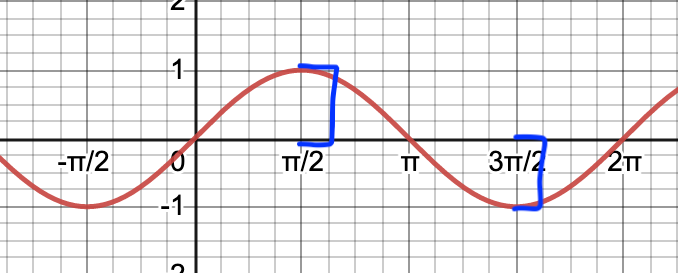
\includegraphics[width=0.6\textwidth]{figures/sine-wave-with-amplitude.png}
    \caption{A sine wave, with the peaks and troughs of the amplitude marked blue}
    \label{fig:sine-wave-with-amplitude}
\end{figure}

\begin{equation}
	y(x,t) = y_m \sin(k(x + \lambda) - \omega t)
	\label{eq:physics-sine-wave}
\end{equation}

The amplitude of a wave ($y_m$) is the magnitude of the maximum displacement of the wave's crest (peak, above 0, or trough, below 0) from its equilibrium position of 0 on the x-axis. As this value is a magnitude, the quantity of amplitude will always be positive, even if it measures the trough of a wave (a negative value, with the amplitude of the wave below 0) instead of the peak (a positive value, above 0). The phase of the wave (defined as the position of a point in time $t$ in a waveform cycle, and in Equation \ref{eq:physics-sine-wave} notated as $kx - \omega t$) will change linearly with a time \texttt{t}, dependent on the oscillation of the wave. Arbitrarily, as a sine wave oscillates between values of $-1$ and $+1$, the wave's amplitude is at value $-y_m$ and $+y_m$ respectively. Thus, the time-dependent nature of the wave's phase will correspond to the oscillation of the wave, with the amplitude determining the extremeness of the displacement of the wave's crest. The wavelength $\lambda$ of a wave is the distance between repetitions of peaks or troughs, and is parallel to the direction of the wave's travel. Finally, the period of a wave \texttt{T} is the time to move through one full oscillation \cite{Halliday_Resnick_Walker_2005}. Due to the nature of a sine wave to follow the unit circle counterclockwise (discussed further in Subsection \ref{subsection:sine-waves}), the sine wave will begin to repeat when its angle $\theta$ (or argument $k$) is increased by $2\pi$. Thus, we have that Equation \ref{eq:sine-wave-period} is equivalent to Equation \ref{eq:physics-wavelength}.

\begin{equation}
	k = \frac{2\pi}{\lambda}
	\label{eq:physics-wavelength}
\end{equation}

It is important to note that there are two types of frequency within sound waves: $\omega$ (angular frequency) and $f$ (temporal frequency). The temporal frequency $f$ of a wave is defined relative to angular frequency $\omega$, as in Equation \ref{eq:physics-freq-eq}. Frequency $f$ is the number of oscillations per unit time, usually measured in Hertz or kilohertz. Angular frequency $\omega$ is the frequency of an arbitrary sine wave as it moves counterclockwise around the unit circle.

\begin{equation}
	f = \frac{1}{T} = \frac{\omega}{2\pi}
	\label{eq:physics-freq-eq}
\end{equation}

The final notable property of waves is the wave forms (the shape of the waves, and different from the term ``waveform'') as the waves move left to right. Alternatively, we could also monitor the wave as it oscillates up and down, but the result is the same: either the displacement of the peaks and troughs of an oscillating wave is perpendicular to the direction of travel of the wave (defined as a \textit{transverse wave}), or the direction of travel of an oscillating wave is parallel to the displacement of the peak of the wave (defined as a \textit{longitudinal wave}) \cite{Halliday_Resnick_Walker_2005}, as in Figure \ref{fig:transverse-wave-longitudinal-wave}. Both wave shapes are also known as \textit{traveling waves}, as they travel from one defined point to another. The sinusoidal, periodic waveforms mentioned in Section \ref{section:waveforms} (and further discussed in Subsections \ref{subsection:sine-waves} through \ref{subsection:triangle-wave}) are transverse waves; as in Figure \ref{fig:transverse-wave-longitudinal-wave}, the black vertical arrows demonstrate the displacement of the sinusoidal wave along the y-axis, while the pink arrow (labeled $\Vec{v}$) shows the movement of the wave along the x-axis.

\begin{figure}[ht]
  \centering
  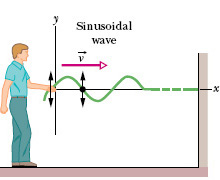
\includegraphics[width=0.3\textwidth]{fig_16_1.jpeg}
  \caption{A sinusoidal wave is sent along the string. A typical string element moves up and down continuously as the wave passes. This too is a transverse wave.} \cite{Halliday_Resnick_Walker_2005}
  \label{fig:transverse-wave-longitudinal-wave}
\end{figure}

Simple tones, such as sine waves and cosine waves, are transverse periodic waves--waves in which the displacement of the wave is perpendicular to the direction of travel of the wave, and which also repeats in a continuous pattern, known as a cycle--that are singular in frequency. These waveforms, as mentioned, are the simple waveforms which compose the building blocks of more complex sounds (waveforms). To demonstrate this concept, we choose the sine wave to serve as an example of the principle of \textit{superposition}, defined as the situation in which two or more waves pass simultaneously through the same region \cite{Halliday_Resnick_Walker_2005}, and several effects (sound alterations) may occur simultaneously, as the net effect is the sum of each wave's individual effects. Suppose we have two waves which are traveling simultaneously through the same stretched string, and let $y_1(x, t)$ and $y_2(x, t)$ be the displacements the string will experience if each wave were to travel alone the wave alone. The total displacement of the string when the waves overlap will then be

\begin{equation}
	y'(x, t) = y_1(x, t) + y_2(x, t)
\end{equation}

Occasionally, multiple sinusoidal waves of the same wavelength and amplitude moving in the same direction may \textit{interfere} with each other, as the superposition principle applies. The resultant wave of this interference depends on the extent to which the waves are in phase/in step with respect to each other. If the phase of both waves are the same (``in phase,'' in which the peaks and troughs of each wave are the same) then the total displacement is doubled from the displacement of each individual wave, resulting in a sound that sounds twice as loud as either of the waves would individually. On the other hand, if both waves are exactly ``out of phase'' (the peaks of one wave is the same as the troughs of the other) then the total interference will result in the cancellation of noise, as each wave will fully cancel the other \cite{Halliday_Resnick_Walker_2005}. This is how much of the ``noise-cancelling'' technology works in headphones and speakers, in which the phases of multiple waveforms combine to cancel each other, resulting in the perception of no noise. As in Equation \ref{eq:noise-cancelling}, suppose $y_1(x, t)$ is the displacement of $y$ of one wave, and $y_2(x, t)$ be the displacement of another wave. 

\begin{equation}
	\begin{aligned}
	y_1(x, t) &= y_m\sin(kx - \omega t) \\ 
	y_2(x, t) &= y_m\sin(kx - \omega t + \varphi)
	\label{eq:noise-cancelling}
	\end{aligned}
\end{equation}

Waves $y_1(x, t)$ and $y_2(x, t)$ have the same angular frequency $\omega$ (and thus also the same temporal frequency $f$, the same angular wave number $k$ (and thus also the same wavelength $\lambda$), and amplitude $y_m$. Both waves travel in the positive direction of the x-axis, at the same speed. The only difference between the two waves is the phase shift $\varphi$, resulting in the two waves being out of phase, and cancelling the noise of the resultant wave. In situations other than perfect ``in phase'' or ``out of phase'' waves, the composite sound will be some sum or difference of the amplitude, wavelength and phase of each of the individual waves.

\subsection{Sine Waves}\label{subsection:sine-waves}
The first of the basic periodic waves is the sine wave, and is the most common type of periodic wave. The sine wave is a signal with only one frequency, and represents the unidimensional motion for any signal with a phase angle that rotates at a constant rate, using both the unit circle in Figure \ref{fig:unit-circle}, and the trigonometric sine function of Equation \ref{eq:sine-wave-equation}. On the unit circle, the trigonometric sine function of a phase angle $\theta$ is defined as the ratio of the length of the opposite side and the hypotenuse of a right triangle, like in Figure \ref{fig:unit-circle} in which the right triangle is outlined in red. The unit circle, with a radius of 1, results in the sine function $sin\theta$ being equal to the y-value in Cartesian coordinates, where the hypotenuse of the right triangle that is formed meets the circle, like in Figure \ref{fig:basic-sine-wave} and Figure \ref{fig:unit-circle}. Here, when $y = 1$ for angle  $\theta = \frac{\pi}{2}$ in the unit circle (Figure \ref{fig:unit-circle}), the y-value of the wave in Figure \ref{fig:basic-sine-wave} corresponds to this y-value, at 1. We can then use this trigonometric sine wave to synthesize a sine wave audio signal. As a sine wave is a continuous periodic wave, in which the wave continues to move until stopped, we must use the sine wave function on the unit circle continuously. Thus, we use the sine function continuously around the unit circle, going counterclockwise. We notice that in the correlation between Figures \ref{fig:basic-sine-wave} and \ref{fig:unit-circle} moving counterclockwise through the unit circle results in the appropriate rise and fall of the sine wave. $\frac{\pi}{2}$ is the highest y-value within the Cartesian plane, and so denotes a peak in the sine wave, while $\frac{3\pi}{2}$ is the lowest, denoting a trough.

\begin{figure}[h]
	\centering
	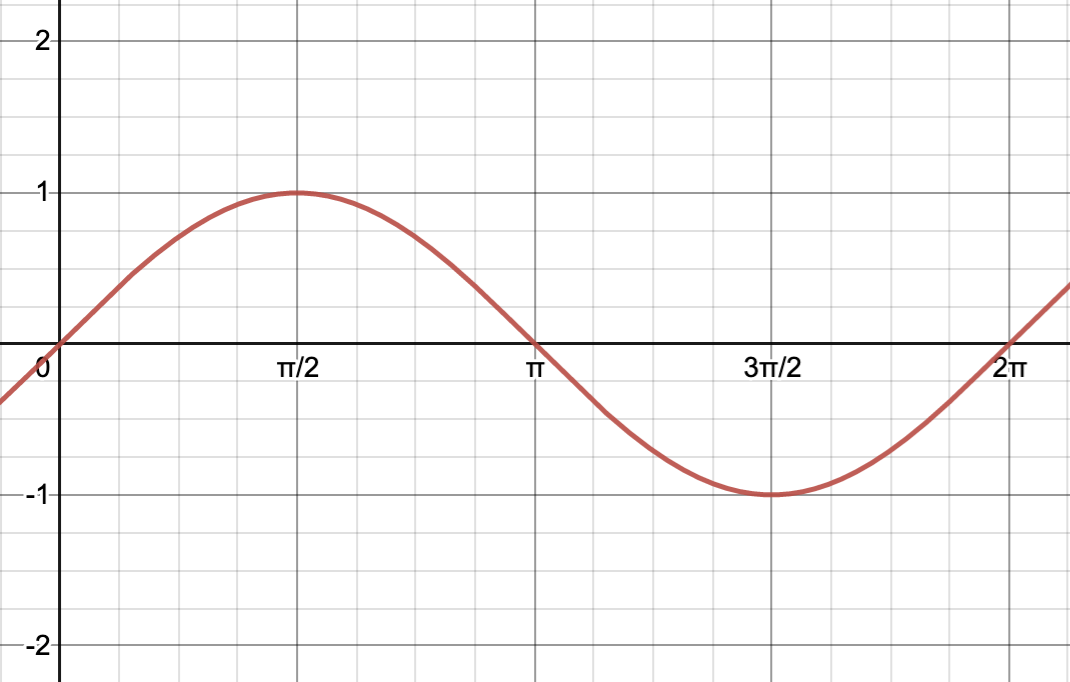
\includegraphics[width=0.5\textwidth]{figures/sine-wave-form.png}
	\caption{A basic sine wave}
	\label{fig:basic-sine-wave}
\end{figure}

\begin{equation}
	y = Asin(B(x + C)) + D
	\label{eq:sine-wave-equation}
\end{equation}

Like with the other periodic waves, sine waves have three important properties: frequency, amplitude, and phase. From the generic function for a sine wave, as in Equation \ref{eq:sine-wave-equation}, we are able to compute the various properties. First, \textit{A} is the sine wave's amplitude. This is defined as the height from the x-axis of the wave to its peak or trough. For our unit sine wave, this value will be 1. Second is the variable \textit{B}, which helps to define the period of the wave, or the distance between one peak and the next, or one trough and the next. With Equation \ref{eq:sine-wave-period}, we see the period is equivalent to taking the total circumference of the unit circle, and dividing it by \textit{B}. Third, the phase shift of a sine wave is denoted by \textit{C}. If the expression is $(x + C)$, then the phase of the sine wave will shift to the left with respect to the value $x + 0$ (with $C = 0$), as the x-value of the wave becomes positive \textit{C}. Otherwise, if the expression is $(x - C)$, then the wave will shift right with respect to the value $x - 0$ ($C = 0$), as x becomes negative \textit{C}. Finally, the variable \textit{D} is equivalent to the vertical shift of the wave. This notates the distance that the wave will shift vertically from its unit circle position. As sine waves are only composed of a fundamental frequency (the lowest frequency found in a wave, for sine waves this will be the frequency of the wave), these waves are most used as pure sound tones. Sine waves are at the center of audio synthesis and sound analysis. Other, more complex, periodic waves can be built using some combination of sine waves. 

\begin{equation}
	\frac{2\pi}{B}
	\label{eq:sine-wave-period}
\end{equation}

\begin{figure}
	\centering
	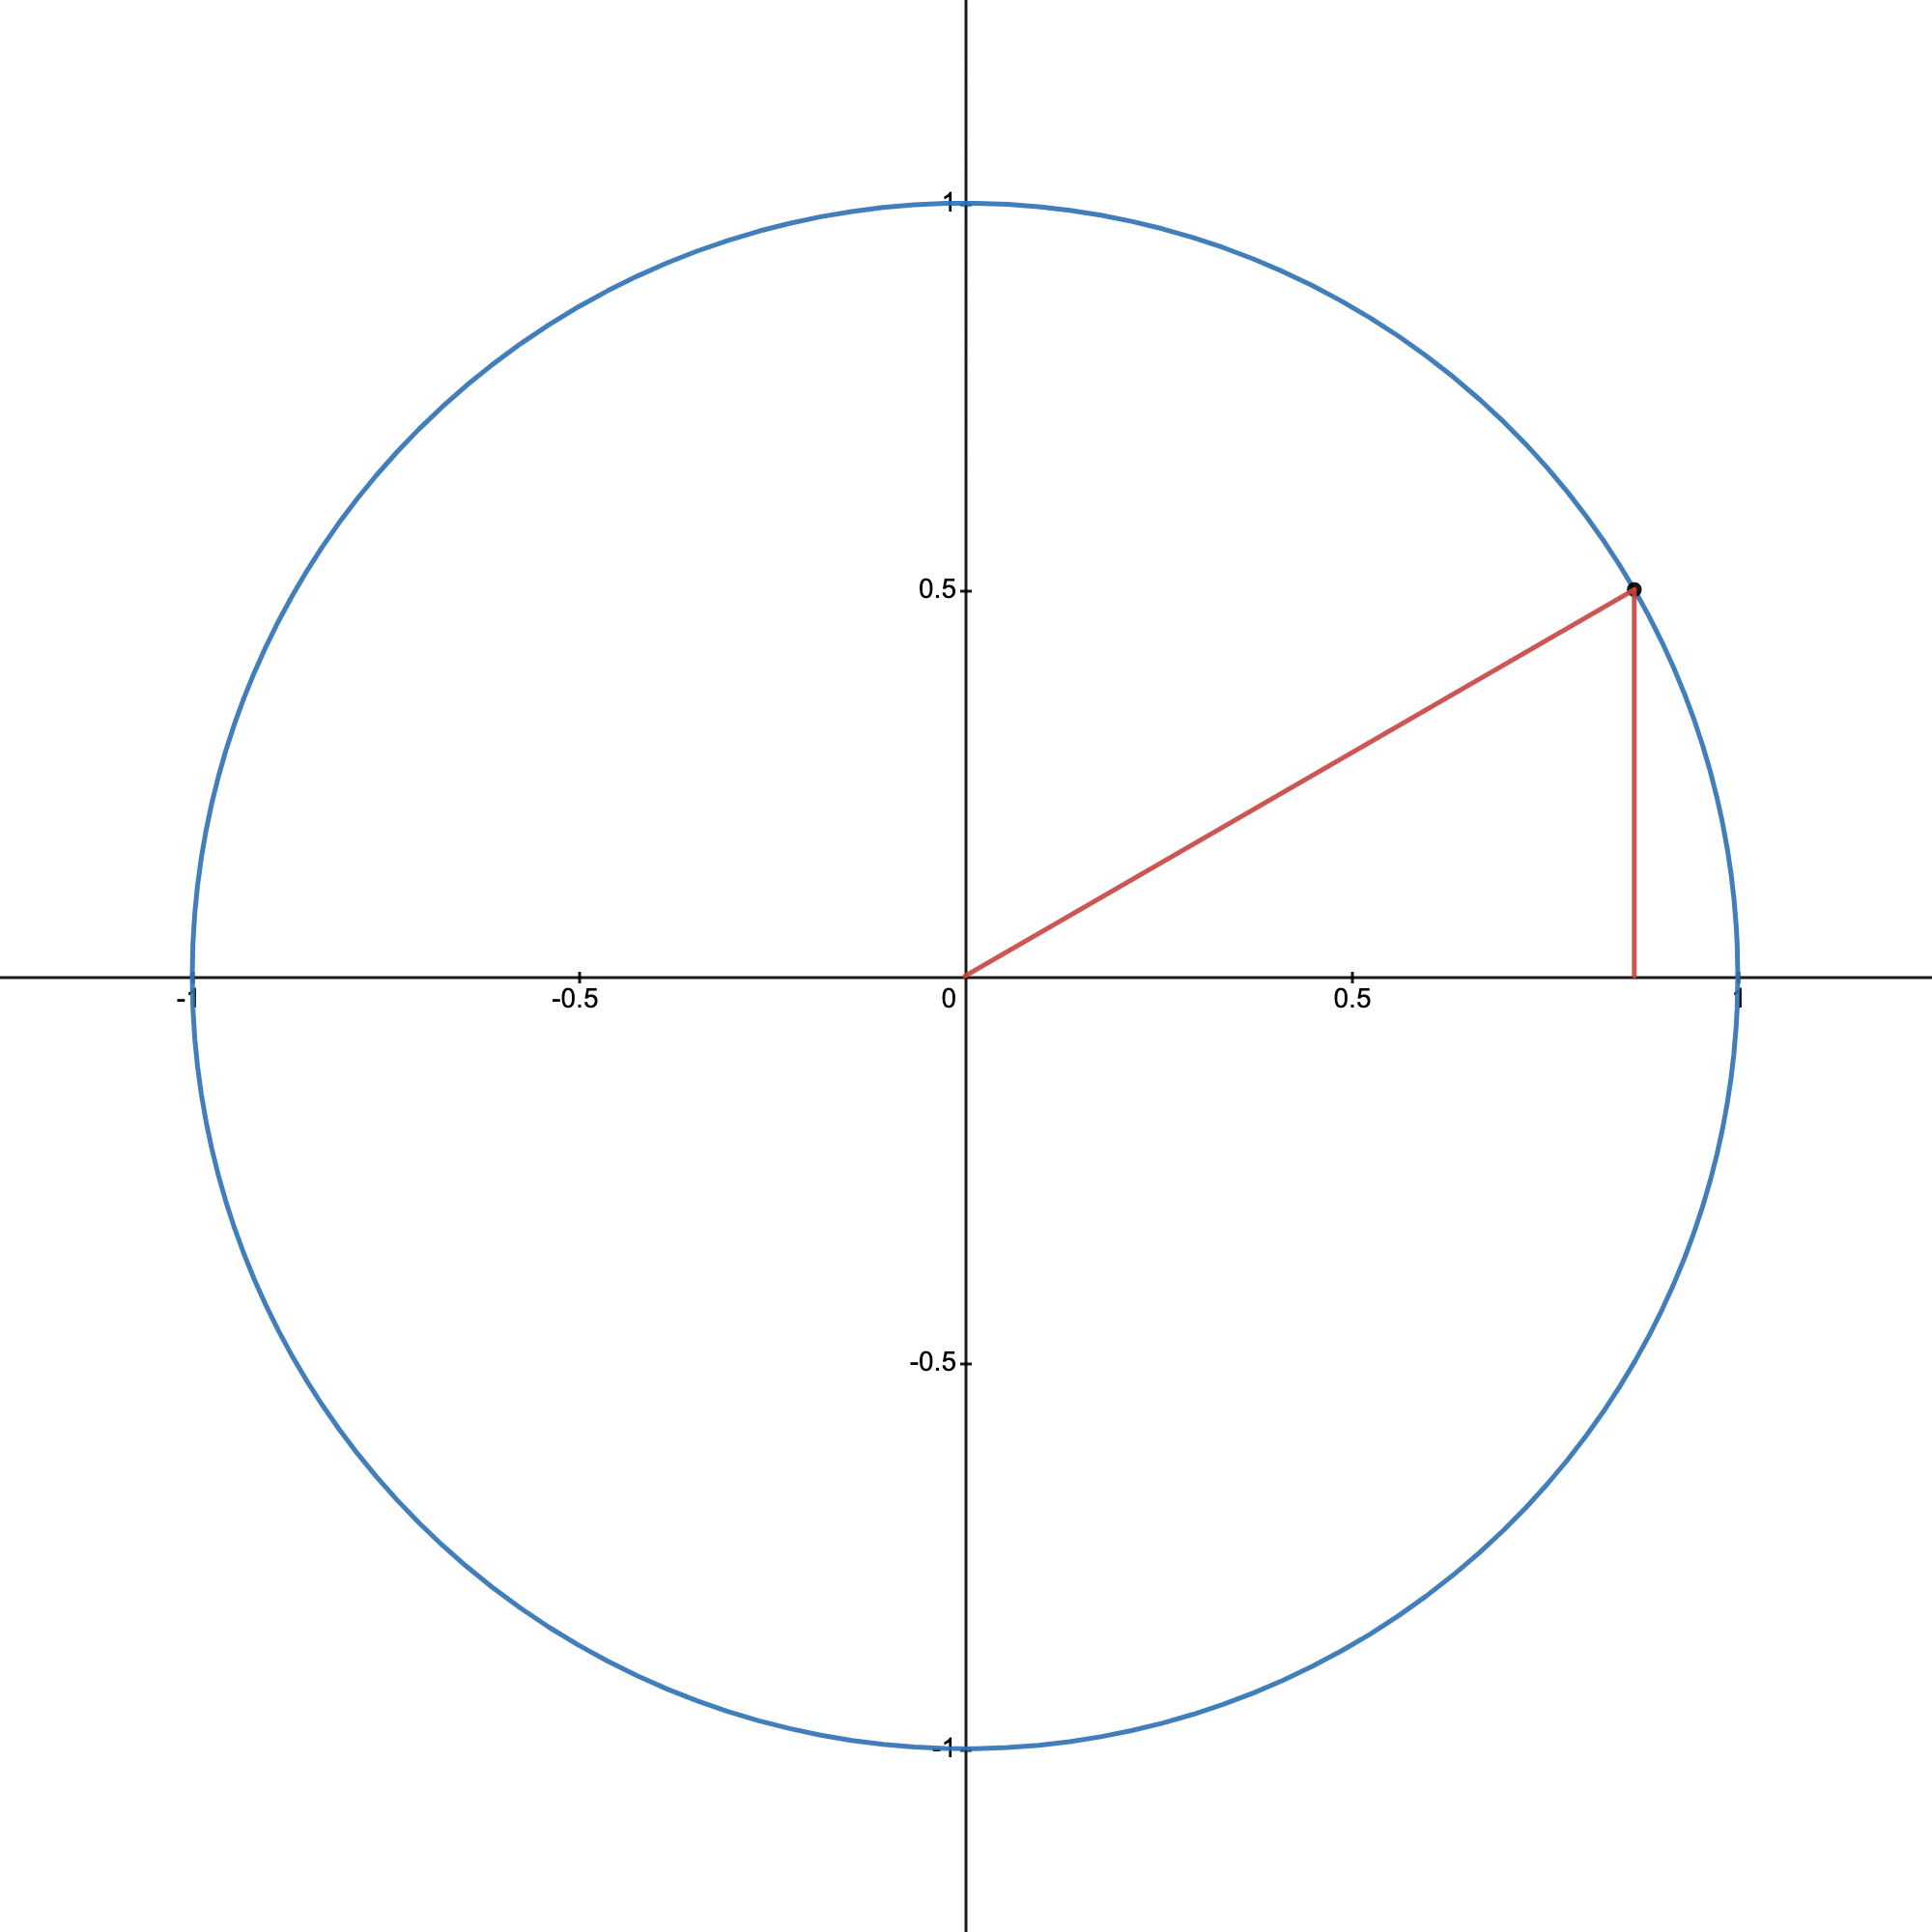
\includegraphics[width=0.5\textwidth]{figures/unit-circle.png}
	\caption{The unit circle}
	\label{fig:unit-circle}
\end{figure}

\subsection{Square Waves}

The square wave is a certain type of pulse wave, which we can represent as a summation of an infinite set of sine waves, similar to how sawtooth waves and triangle waves can also be a summation of sine waves. \textit{Additive sythesis}\footnote{Further defined in section \ref{section:mod-synth-history}.} is one method we can use to create square waves, sawtooth waves, and triangle waves, and so we notice that the functions for these waves have similar periodic equations. Through additive synthesis, we layer multiple sine waves, such that the composite wave is typically a square wave, sawtooth wave, or triangle wave. In the equation for a square wave, we have variables $f$ (frequency), $A$ (amplitude), and $n$ number of harmonics, let $f(x)$ be an arbitrary square wave as a function of time $t$ in Equation \ref{eq:square-wave-summation}. Like with triangle waves, odd harmonics (or waves in which only odd values are valid) are the only valid values for this type of periodic waveform. This causes a non-smooth waveform, as unlike the smooth oscillations of a sine wave, odd waveforms ramp upwards to the peak amplitude height, and downwards to the lowest amplitude trough. This results in a sharper sound. Then, positive $i$, in Equation \ref{eq:square-wave-summation}, will always be odd, such that these harmonics create the square wave of Figure \ref{fig:square-wave}.

\begin{figure}[ht]
  \centering
  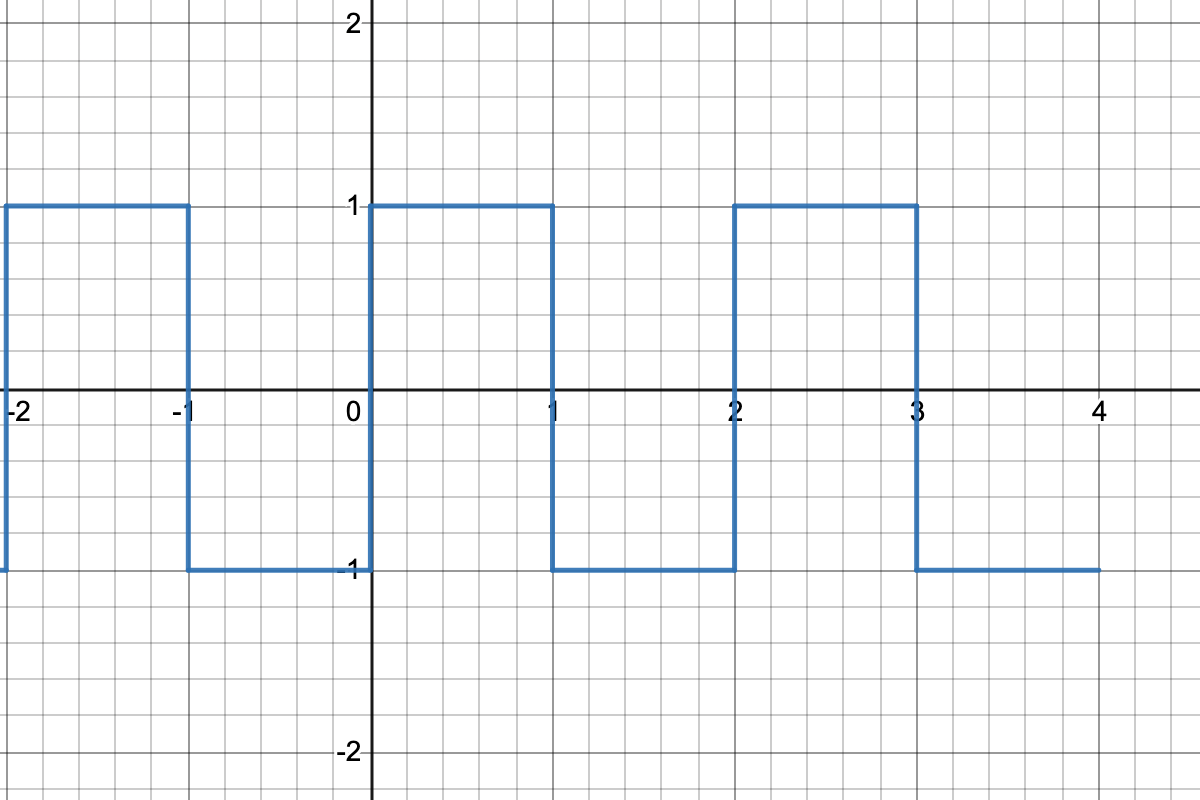
\includegraphics[width=0.5\textwidth]{square-wave.png}
  \caption{A basic square wave}
  \label{fig:square-wave}
\end{figure}

\begin{equation}
	f(x) = A\sum_{i=1}^{\infty}\frac{\sin(2\pi nft)}{n}
	\label{eq:square-wave-summation}
\end{equation}

There are three properties of the square wave which we can manipulate: the frequency $f$, amplitude $A$, and phase (altering $2\pi nft$ from Equation \ref{eq:square-wave-summation}), from the summation equation for square waves (Equation \ref{eq:square-wave-summation}). First, the amplitude value $A$ (similar to variable $A$ of Equation \ref{eq:sine-wave-equation}) will alter the height (displacement of $y$) of the wave's peak and trough from the x-axis. This will change the volume we perceive the square wave to be at. In Figure \ref{fig:square-wave}, the square wave pictured is a unit square wave, in which the amplitude will be 1. Second, is frequency $f$, which defines the period of the wave. A larger $f$ (like with variable $B$ of Equation \ref{eq:sine-wave-equation}) value will cause the value of the period also becoming larger, thus resulting in a sound with a higher pitch. Third, the phase shift of the square wave will be denoted by changes to the expression $2\pi nft$ (similar to the usage of variable $C$ of Equation \ref{eq:sine-wave-equation}). Like with changes to $C$ of the sine wave equation, alterations to a square wave's phase involves adding or subtracting a value to time \texttt{t} \cite{Wellesley_College_Staff_2021}. For instance, to adjust the phase of a square wave to sound 0.5 seconds delayed, we would alter $2\pi nft$ by doing the following

\begin{equation*}
    f(x) = A \sum_{i=1}^{\infty} \frac{sin(2\pi nft - 0.5)}{n}
\end{equation*}

As the value of this modification to time \texttt{t} is negative ($-0.5$), the wave will shift right, and sound delayed. This is similar to the negative \textit{C} value of the sine wave function, since a positive value will result in the square wave to shift to the left (in respect to a phase shift value of 0) and sound early.

The sound produced by a square wave is one that is harsh and bright, that is, a sound which has many frequencies in the higher frequency ranges (bright), and lacks much of the lower end of the frequency ranges (harsh). In combination, this results in a sound that becomes grating to hear after some time, and introduces listening fatigue. These waves also only contain odd harmonics, so are most used to simulate the sounds of woodwinds and reeds \cite{Dowsett_2016}. 

% \begin{equation}
% 	sgn (x): \begin{cases}
% 		-1 & \textrm{if } x < 0, \\
% 		0 & \textrm{if } x = 0, \\
% 		1 & \textrm{if } x > 0
% 	\end{cases}
% 	\label{eq:sgn-function}
% \end{equation}

% \begin{figure}[ht]
%   \centering
%   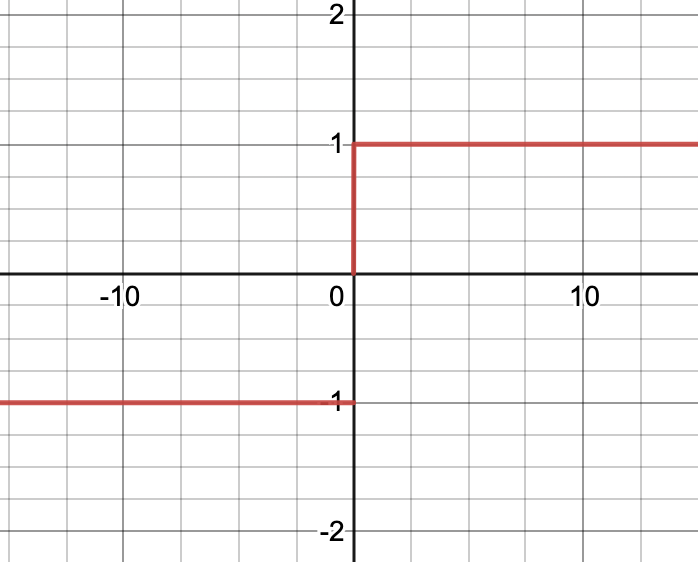
\includegraphics[width=0.5\textwidth]{sign-function.png}
%   \caption{A sign function}
%   \label{fig:sign-function}
% \end{figure}

% In a square wave equal to Equation \ref{eq:square-wave-function}, the function $sgn(x) = 1$ when the sinusoidal is positive, $sgn(x) = -1$ when negative, and $sgn(x) = 0$ when the sinusoidal is equivalent to 0. Other aspects of the formula can be altered, similarly to how the function for the sine wave is modified, to produce sound changes. The variable $f$ can be modified like how a period for a sine wave is (variable $B$), in which a larger value, as long as the new value is odd, is able to cause a different frequency result over time \texttt{t}. Amplitude can be increased by multiplying our $A$ value, in Equation \ref{eq:square-wave-function} notated as $sgn$, by some arbitrary odd value. This will increase the value of the amplitude, or the value of $x(t)$ to some other value greater than $+1$ and less than $-1$. Finally, we are also able to modify the period of a square wave, multiplying an odd value by our variable $B$, or $\sin(2\pi)$ \cite{Case_2007}.

\subsection{Sawtooth Waves}
Like with the square wave, one notable characteristic of the sawtooth waveform is that is it a non-sinusoidal wave, and resembles the teeth of a plain-toothed saw. Additionally, as in Figure \ref{fig:basic-sawtooth-wave}, a sawtooth wave will ramp upwards to a peak amplitude height as the amplitude increases linearly, reaches a set maximum volume, then sharply drop to its trough, or the set minimum value (typically 0). This sudden drop (the non-linear component of sawtooth waves) to the set minimum value for amplitude results in the wave beginning a new period, or new cycle. This is defined by Equation \ref{eq:sawtooth-summation-function}, in which multiple sine waves create a sawtooth wave \cite{Tarr_2019}. We notice that this equation is similar to that of the square wave function, with a small difference: the expression $2\pi fnt$ is no longer a fraction over $n$ to create a sawtooth wave. This difference is seen in both Figure \ref{fig:square-wave} and Figure \ref{fig:basic-sawtooth-wave}, in the ways in which each wave descends from its peak to its trough, and the value of time \texttt{t} which the wave spends at its peak or trough.

\begin{figure}[ht]
  \centering
  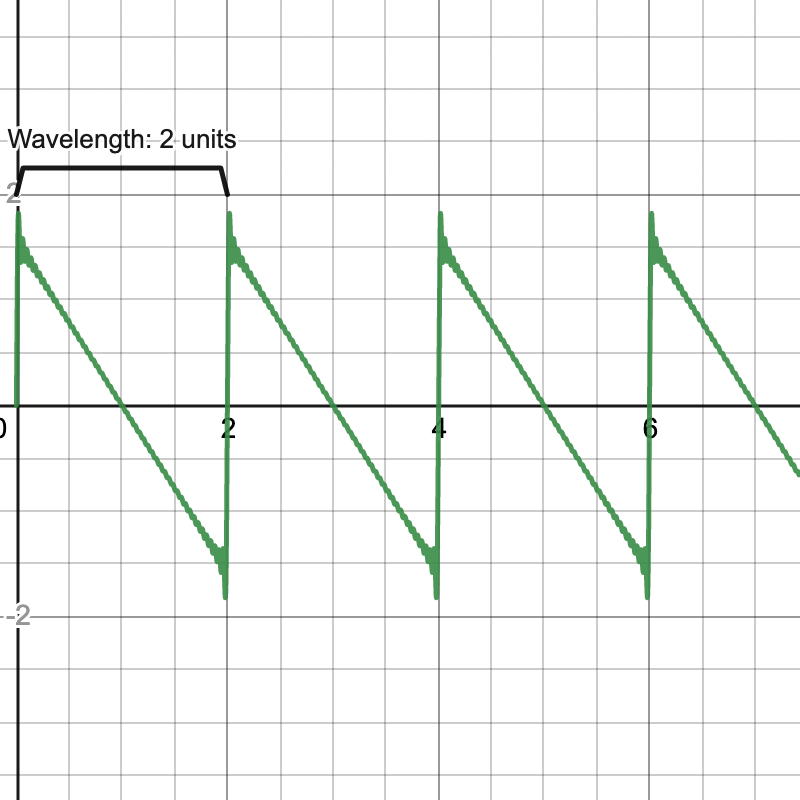
\includegraphics[width=0.3\textwidth]{figures/sawtooth-wave.png}
  \caption{A basic sawtooth wave}
  \label{fig:basic-sawtooth-wave}
\end{figure}

\begin{equation}
	f(x) = \sum_{n=1}^{\infty} \frac{A}{n}\sin(2\pi fnt)
	\label{eq:sawtooth-summation-function}
\end{equation}

In a sawtooth wave, we again have three properties we can easily manipulate: amplitude ($A$), frequency $f$, and phase shift (the expression $2\pi fnt$). Each of these variables have their sine wave function equivalent from Equation \ref{eq:sine-wave-equation}. Amplitude $A$ equals the sine wave function variable $A$, frequency $f$ is equivalent to variable \textit{B}, and phase shift $2\pi fnt$ is the same as variable $C$. The amplitude $A$ will alter the sawtooth wave's amplitude, adjusting the distance from a peak or trough to the x-axis, and thus also the perceived volume. Frequency $f$ defines the period of the sawtooth wave, in which a higher value $f$ will cause a higher number of cycles to occur, and the perceived pitch to rise. Finally, the phase shift $2\pi fnt$ works similarly to how it does in the square wave function, in which an addition or subtraction to time \texttt{t} affects how early or delayed the resulting sound will be.

% Alternatively, the function for a sawtooth wave can be expressed as the summation of an infinite set of sine waves (which combined, can create a singular sawtooth wave). For Equation \ref{eq:sawtooth-summation-function}, let $f(x)$ be a sawtooth wave as a function of $t$ time in seconds, with frequency $f$, amplitude $A$, and $n$ many harmonics \cite{Wellesley_College_Staff_2021}. Adjustments to this function can easily be done through modifying the values of $f$ and $A$.

% , as in Figure \ref{fig:basic-sawtooth-wave}, creating Equation \ref{eq:sawtooth-sinusoidal-function}, with $frac(x)$ referring to what is in Equation \ref{eq:sawtooth-piecewise-function}, as the fractional part of the equation. 

% \begin{equation}
% 	S(x) = Afrac(\frac{x}{T} + \phi)
% 	\label{eq:sawtooth-sinusoidal-function}
% \end{equation}

% \begin{equation}
% 	frac(x) = x - \lfloor x \rfloor
% 	\label{eq:sawtooth-piecewise-function}
% \end{equation}

% The function $frac(x)$ gives the fractional (or non-integer) part of an arbitrary real number $x$ \cite{Weisstein}. Let $\lfloor x \rfloor$ be defined as the greatest integer which is less than or equal to a real number $x$. Thus, the fractional part of $x$ will be $frac(x) = x - \lfloor x \rfloor$, as seen in Equation \ref{eq:sawtooth-piecewise-function}. For both nonnegative and negative real numbers, $frac(x)$ will be a positive value.

Within physical musical instruments, sawtooth waves are most often found within the playing of a string instrument, such as the violin, viola, or cello. As a bowed string oscillates, the bow alternates, in an up-down motion, sticking to the string. The bow will drag the string along as it plays, then slips to allow the string to return to its neutral position \cite{Kapur_Cook_Salazar_Wang_2015} Thus, the nature of the sawtooth wave gives it a bright and energetic sound, and contains both even and odd harmonics, creating a relatively smooth oscillating sound. Due to this, sawtooth waves will be used for a variety of instruments, such as strings, brass, pads, and basses \cite{Dowsett_2016}. 


\subsection{Triangle Wave}\label{subsection:triangle-wave}

A triangle wave is also a non-sinusoidal waveform, named for its triangular shape. Like with square waves, this type of wave only contains odd harmonics, creating a sound which is not smooth in its oscillation from peak to trough and back again. It also shares similarities to the sawtooth wave with the amplitude of the wave increasing linearly to a set maximum value from 0, reaching this maximum value, then decreasing back to 0. However, there is a small difference in the two waves. While a sawtooth wave will decrease in amplitude from its set maximum value back to 0 immediately (in a non-linear way, as seen in Figure \ref{fig:basic-sawtooth-wave}) the amplitude of a triangle wave will decrease linearly upon achieving the set maximum amplitude value, as in Figure \ref{fig:triangle-wave}, until the minimum value is reached \cite{Tarr_2019}.

\begin{figure}[ht]
  \centering
  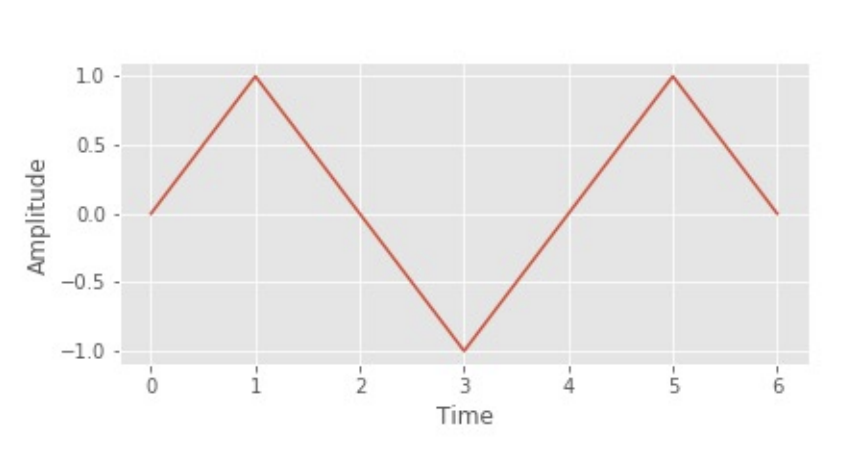
\includegraphics[width=0.4\textwidth]{triangle-waves.png}
  \caption{A basic triangle wave}\cite{Wellesley_College_Staff_2021}
  \label{fig:triangle-wave}
\end{figure}

As with the other waveforms mentioned, triangle waves can be written as the summation of sine waves. Let $f(x)$ be any triangle wave as a function of time $t$ in seconds, with frequency $f$, $n$ number of harmonics (which can simply be thought of as cycles) and amplitude $A$. Thus, Equation \ref{eq:triangle-summation-function} will indicate the cycles of a triangle wave. The equation for the triangle wave is similar to those for the other two waveforms (square waves and sawtooth waves), with the primary differences being the multiplication of $(-1)^i$ and the amplitude $A$ being divided by $\frac{n}{2}$. So trough adjustments to variables $f$, $A$ and $2\pi fnt$, various sound output changes can be achieved. First, the amplitude $A$ will be divided by $\frac{n}{2}$ (the square of the number of harmonics $n$), and is similar to the variable $A$ of Equation \ref{eq:sine-wave-equation}. This value determines the amplitude of the triangle wave, and thus also the perceived volume of the wave. Second, frequency $f$ defines the period of the wave, similarly to variable $B$ of Equation \ref{eq:sine-wave-equation}, affecting the number of cycles which appear and also the perceived pitch of the wave. Finally, the phase shift of $2\pi fnt$ acts similarly as it does in the square wave and sawtooth wave functions. A value added to $2\pi fnt$ results in the wave sounding early, while a subtraction from $2\pi fnt$ causes the wave to sound delayed. 

% \begin{equation}
% 	f(x) = \frac{2}{\pi}sin^{-1}\lceil sin(\pi x) \rceil
% 	\label{eq:triangle-wave-function}	
% \end{equation}

\begin{equation}
	f(x) = \sum_{i=1}^{\infty} (-1)^i \frac{A}{n^2} \sin(2\pi fnt)
	\label{eq:triangle-summation-function}
\end{equation}

Triangle waves are also ``soft'' sounding waveforms, which decrease in sound faster than some other types of waves. This results in triangle waves being used to simulate piano and flute sounds, as well as other instruments which rely on the quick decay of a note \cite{Dowsett_2016}.

\section{Representing Sound Digitally}

We now understand the physics and mathematics behind sound waves. However, sounds in real life are not composed of simple pure waveforms; sounds in the world around us are made up of multiple harmonics and frequencies layered on top of one another to produce the composite sound which we hear. Sound, like electricity and light, is a form of energy in which molecules in air vibrate and move in a wave pattern. This wave pattern produces the sound waves \cite{Au-Yeung_2021}. Air is able to support multiple sound waves simultaneously, explaining our ability to hear different sounds at the same time. This sound energy is dispersed outwards from the sound source, and will continue to move until the molecules run out of energy, as the energy weakens the further it moves away from the sound source (or the sound \textit{attenuates}). The sound energy is transferred between molecules, as each molecule moves from an original resting point, transfers energy to another molecule as they collide, then returns to its resting point, as in Figure \ref{fig:graphical-rep-vs-physical-sound}. This molecule movement is the oscillation of sound. Molecules become closer together when vibrating, and crowd together in certain places, and thus there are fewer molecules in other places. This visualization of crowds of molecules can be done as a wave, with the peak of a sound wave indicating that there are more molecules together in space (compression of air molecules), and the trough of a sound wave indicating there are fewer molecules (rarefaction) \cite{Toft_2020}. Typically, sound is visualized in a graphical format, with peaks and troughs to a wave rather than drawings showing the compression and rarefaction of air molecules. 

\begin{figure}
  \centering
  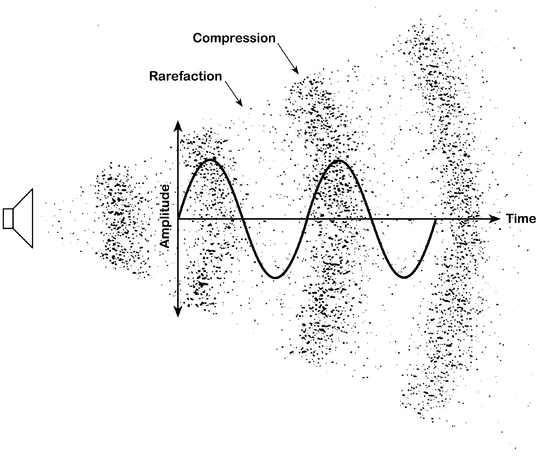
\includegraphics[width=0.4\textwidth]{graphical-rep-vs-physical-sound.jpeg}
  \caption{A graphical representation of sound, vs its physical phenomenon}\cite{Toft_2020}
  \label{fig:graphical-rep-vs-physical-sound}
\end{figure}

Through this periodic nature of waves, the repetitions create what we will recognize to be musical sound, but lacking the specific tonality and timbral qualities of specific instruments. Musical instruments generate a composite set of frequencies, arranged as a layered set of harmonics above the fundamental frequency (the lowest frequency which is played). Thus, the fundamental frequency will be the pitch of the note, and the additional harmonics (also known as overtones) will lie above this pitch and add the tonality or timbre of the note \cite{Toft_2020}. This is what differentiates pure sound waveforms from notes generated from musical instruments, as pure sound waveforms all have pitch, but lack specific timbral quality.\footnote{This is what gives pure sound waveforms their name, ``pure tones,'' as each of these waveforms has pitch but no timbre.} Another factor which dictates what a sound wave will be perceived as is the amplitude of a wave, which will be further discussed in Section \ref{section:manip-waves}.

To get from an analog sound wave to a digital sound signal, we must sample the continuous analog wave into its digital representation. Current technology is incapable of working with a complete, continuous analog sound wave, as it is made up of infinite points. To counter this, we must sample the analog sound wave to convert it into a digital signal, which produces a finite set of discrete points. Together, these points will allow us to visualize an analog sound wave in the digital domain. To sample an analog audio signal is to measure the signal at different points in time, while recording the physical property of that signal as a number. Typically, voltage is measured, which can be transmitted into a stream of numbers \cite{Anderson}. While an audio signal or sound is a continuous set of values, which are able to be displayed on an oscilloscope (a tool to show oscillations) as a waveform, the digital ``signal'' is a series of numbers, representing various discrete values from the continuous wave. These numbers will represent the values of an audio signal at specific points in time, and are known as \textit{samples} \cite{Russ_2012}. The sampling process to convert from analog (physical) waves to a digital signal involves two steps:

\begin{enumerate}
	\item The audio signal is ``sampled'' in which data is captured at defined intervals from one continuous audio signal.
	\item The sample values are converted into discrete numbers.
\end{enumerate}

Once the sampling stage is complete, this sampled data will be digitally scaled down to a target data rate and bandwidth for further processing and storage. The process of sampling will typically produce numbers which are an incomplete representation of the original audio sound, but through careful sampling, this amount of incompleteness can be made insignificant. This same process can be reversed to convert from a digital signal to an analog one, and is known as ``sample replay.'' Sample replay also has three stages and serves as the basis for digital synthesizers, as the conversion from digital signal to analog wave produces the sound that is heard.

% \begin{enumerate}
% 	\item A number is presented to an input port.
% 	\item This number is converted into an analog signal.
% 	\item The analog value forms part of an audio signal.
% \end{enumerate}

Analog sound exists in two dimensions: time (a period of each wavelength) and space (the displacement of each waveform from the atmospheric pressure). So it makes sense that to convert from analog audio to digital signals, we use these two dimensions: time (to convert a continuously moving analog audio wave to the digital domain, through the use of a \textit{sample rate}) and space (in the digital domain, this will be in terms of the \textit{bit depth}). 

\textit{Sample rate}, or \textit{sample frequency}, is the number of samples which are captured per period (which is commonly measured in Hertz). Typically, digital audio samples of analog audio waves are taken at 8,000 times per second, or more \cite{Zjalic_2021}. Occasionally, a sound will be sampled that is at a frequency rate higher than 8,000 and the system doing the sampling is unable to identify two points on the waveform to understand the period. Harry Nyquist (1879-1976), a Swedish physicist and electrical engineer, solved this problem through the \textit{Nyquist frequency} \cite{Zjalic_2021} (or \textit{folding frequency}). Nyquist discovered that in order for an analog audio wave to be accurately represented by a digital signal, and thus also the system which is sampling the audio wave, the wave must be sampled at least twice per wavelength, known as the \textit{Nyquist Theorem} (or \textit{Nyquist-Shannon} theorem) \cite{Zjalic_2021} and visualized in Figure \ref{fig:nyquist-sampling-theorem}. Within the first part of Figure \ref{fig:nyquist-sampling-theorem}, the signal is sampled perfectly at $2x$ the Nyquist Frequency. This allows the relevant discrete numbers to be captured, to fully represent the wave. The second image of Figure \ref{fig:nyquist-sampling-theorem} is sampled at a rate which is less than $2x$ the Nyquist Frequency ($1.5x$ for the middle image), managing to capture less than half the needed discrete values to fully represent the wave. Thus, for a given sample rate, the highest frequency within a system cannot exceed half this sample rate. In other words, the Nyquist frequency is the frequency at 50\% of the sample rate. Otherwise, for a frequency which does not satisfy the requirements for the Nyquist Theorem, a phenomenon called ``aliasing'' would occur. Aliasing is the phenomenon in which signals that exceed half the sample rate are misrepresented as ``alias signals'' leading to the wave to be indistinguishable, and incorrect frequency and amplitude values to be obtained. The middle image of Figure \ref{fig:nyquist-sampling-theorem} describes the concept of aliasing, in which the wave is sampled at only $1.5x$ the Nyquist Frequency, and alias discrete points are introduced. These alias points, which make up an ``alias signal,'' are not a true representation of the original signal. An ``anti-aliasing'' filter, or Nyquist filter, would then typically be applied to the signal before sampling occurs, to act as a low-pass filter with a cut-off at the Nyquist frequency. 

\begin{figure}[H]
  \centering
  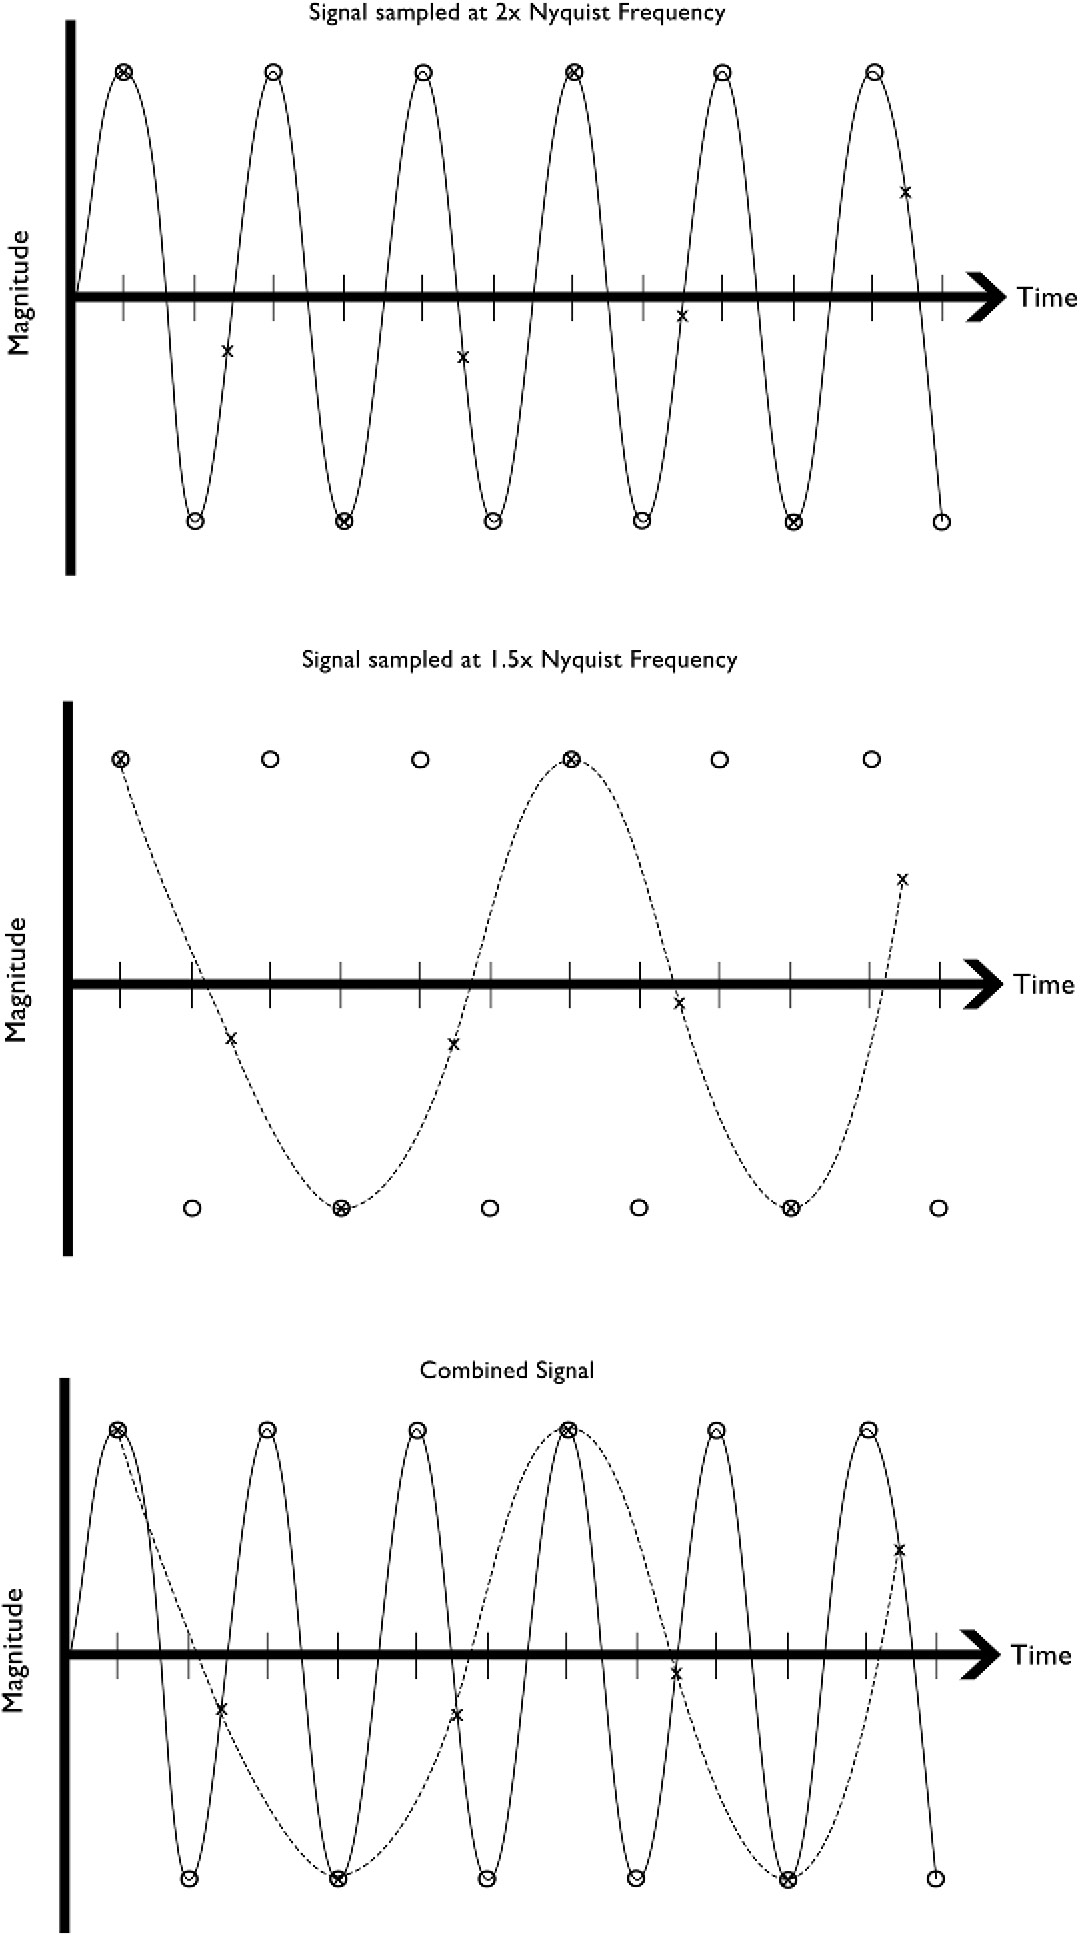
\includegraphics[width=0.5\textwidth]{nyquist-sampling-thoerem.jpeg}
  \caption{The Nyquist sampling theorem visualized. Upper: Signal sampled at 2x Nyquist frequency, Middle: Signal sampled at 1.5x Nyquist frequency (and thus aliasing and not a true representation of the original signal), Bottom: Signal containing both accurate and aliasing components}\cite{Zjalic_2021}
  \label{fig:nyquist-sampling-theorem}
\end{figure}

This sampling process using the Nyquist frequency and anti-aliasing filter is commonly used in digital audio systems (both for professional and consumer usage). Another tool that is commonly used to improve the anti-aliasing filter is \textit{oversampling} \cite{Huber_Runstein_2018}. Oversampling can increase the effective sample rate between 12 and 128 times the original rate, with three primary reasons for this process.

\begin{enumerate}
	\item Physical anti-aliasing filters--like those found in analog-to-digital converters (ADC)--can be expensive, and difficult to design properly. So by increasing the effective sample rate, and the ceiling for this sample rate, a simpler and less-costly filter can be used.
	\item Oversampling typically results in a higher-quality conversion, for both analog-to-digital (A/D) and digital-to-analog (D/A) conversion.
	\item Multiple samples are usually taken of a single sample rate, and so the average noise level will be lower.
\end{enumerate}

\textit{Bit depth} is defined as the discrete values which are available within the digital system, representing the magnitude of a continuous electrical signal \cite{Zjalic_2021}, in the form $log_2{x}$. These levels can become exponentially large, and so \textit{quantization} is used to process data from a broad range into values within a smaller range. It will convert the levels of a continuous analog signal, as the signal after sampling is still in the analog domain, into binary digits (bits). Using bits will allow us to be able to manipulate and store audio data digitally. After sampling the amplitude of an analog audio wave at various precise intervals, we are able to output this amplitude level in its equivalent in bits, which represent the originally sampled amplitude level, known as \textit{bit rates}. The bit ``rate'' can then be defined as the amount of data stored or transmitted per second of time, or in Equation \ref{eq:bit-rate}, measured in kbps \cite{Zjalic_2021}. In general, the higher the value of the bit rate, the higher the quality of the audio data that is stored, since there is more data to represent the captured sound available.

\begin{equation}
	\textrm{bit rate (bits per second)} = \textrm{sample rate (Hz) x } \textrm{bit depth x } \textrm{number of channels}
	\label{eq:bit-rate}	
\end{equation}

Increasing the number of channels will increase the \textit{stereo width} of a sound, or how ``wide'' it is. \textit{Stereophonic sound} (or \textit{stereo}) is a method of sound reproduction which recreates a multi-directional, 3-dimensional audible perspective. Typically, this is achieved by using two independent audio channels fed through a configuration of two loudspeakers (or stereo headphones) to create the impression of sound heard from various directions, similar to how we naturally hear \cite{Au-Yeung_2021}. Different sounds will play from the left speaker or headphone than from the right, thus creating the illusion that the audio is coming from multiple directions. Stereo sound will be used most often in film and music, where there is a combination of music, vocals, and other sounds. \textit{Monophonic sound} (\textit{mono}) occurs when two loudspeakers, or stereo headphones, play the same sound equally \cite{Au-Yeung_2021}. Both the left and right speaker or headphone will play identical audio. Mono sound will typically be used for radio talk shows, telephone calls, or other times when there is a focus on vocals.

From our original three stages of converting analog sound to digital signals, we can now specify the processes which occur in each stage \cite{Huber_Runstein_2018}. 

\begin{enumerate}
	\item Sampling analog audio wave amplitude levels at precise intervals in time.
	\item Converting these samples into the digital bit value (typically a 16-bit length), which most accurately represents the amplitude levels.
	\item Storing these sample equivalents (the bit values) within digital memory.
\end{enumerate}

Upon playback, the bits are then converted back into analog amplitude values, at precise intervals in time, allowing for the originally recorded amplitude values to be re-created, processed, and played back \cite{Huber_Runstein_2018}. 

\section{Manipulating Sound Waves}\label{section:manip-waves}
As previously mentioned in Section \ref{section:modular-synth-what-is}, modular synthesis involves sending an audio signal through patches or modules in a linear format to achieve the desired sound output changes. To explain how these changes occur to a sound wave, we arbitrarily choose the simple sine wave as an example, as in Appendix \ref{appendix:music-theory-terms}. 

\begin{figure}[H]
	\centering
	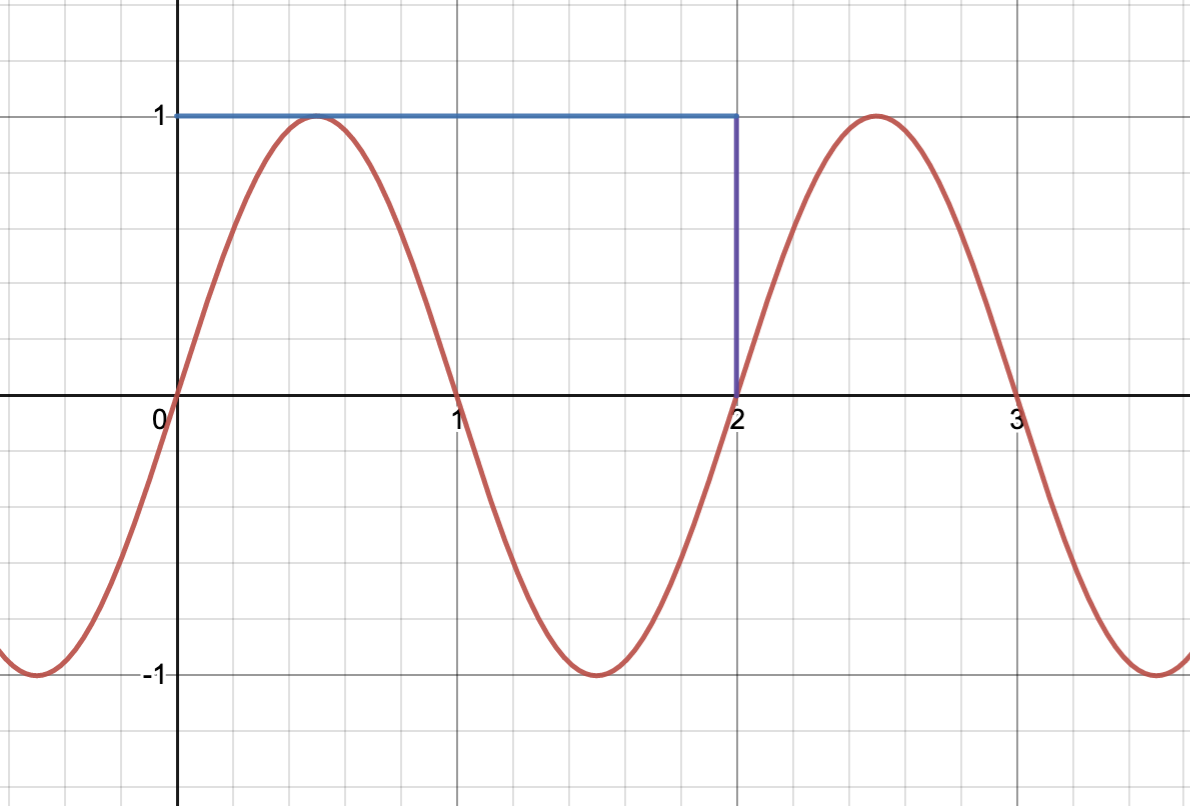
\includegraphics[width=0.5\textwidth]{figures/sine-wave-period-amplitude.png}
	\caption{A basic sine wave, with period demarcated in blue, and amplitude in purple}
	\label{fig:sine-wave-period-amplitude}
\end{figure}

\begin{equation}\label{eq:full-sine-wave-equation}
	y(t) = A \sin(2\pi ft + \varphi)
\end{equation}

Sine waves are a waveform which is a function of time \texttt{t} with variables $A$, $\varphi$. $A$ is the wave's amplitude, which determines the peak deviation from zero. The frequency is $f$, and $\varphi$ is the wave's phase, which specifies (in radians) where in its cycle the wave's oscillation is at time $t$ \cite{Kirk_Hunt_2013}. When $\varphi$ is not equal to zero, the wave itself will appear to be shifted by the value equal to $\varphi$, which is known as a wave's \say{phase shift.} A negative value will represent a delay in sound, while a positive value will represent an advance in the heard sound.

Thus, there are three primary parameters when manipulating audio (or a simple waveform); amplitude, frequency, and phase can all be modified at various points to affect the audio output. The first, amplitude, will determine the volume of the wave's sound. The larger the distance between zero and the wave's peak, the louder the human ear will perceive the sound to be \cite{Zjalic_2021}. In Figure \ref{fig:sine-wave-period-amplitude}, amplitude is colored purple, and we see it has a value of 1 (the default value of amplitude of a sine wave from the unit circle), as $A$ does in Equation \ref{eq:full-sine-wave-equation}. By changing the value of $A$ to either $\frac{1}{2}$, or $2$, the peak of the wave will change accordingly, becoming larger or smaller depending on the set value of $A$. This change is reflected in the sound we can hear, as like in Figure \ref{fig:half-sized-sine-wave} and Equation \ref{eq:half-sized-sine-wave}, the volume of this sine wave is halved. Thus, volume ranges can be between soft (at a barely audible \textit{pianissimo}) with an amplitude $A = \frac{1}{2}$, or loud (\textit{fortissimo}), with $A = 4$, for instance.

\begin{equation}\label{eq:half-sized-sine-wave}
	y(t) = \frac{1}{2} \sin(\omega t + \varphi)
\end{equation}

\begin{figure}[ht]
	\centering
	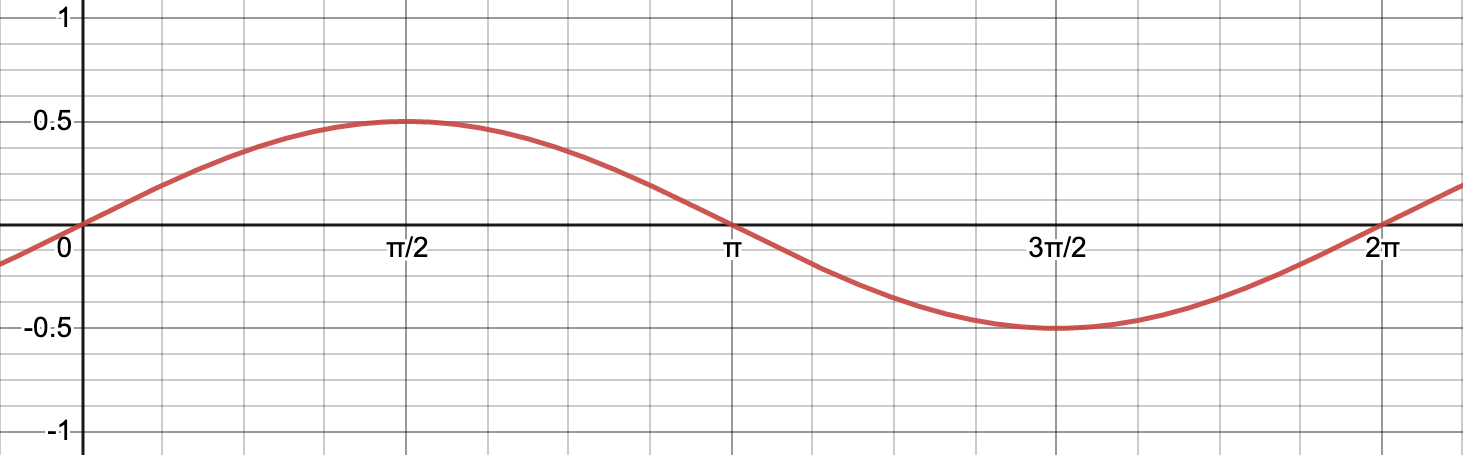
\includegraphics[width=0.5\textwidth]{figures/half-sized-sine-wave.png}
	\caption{A sine wave, with an amplitude of $\frac{1}{2}$}
	\label{fig:half-sized-sine-wave}
\end{figure}

The second option commonly used to manipulate audio is to change an audio signal or wave's frequency. For sound and audio manipulations, the frequency component determines a sound's \say{color,} or \say{timbre.} It is the property of a waveform which determines the output sound's pitch. (Refer to Appendix \ref{appendix:frequency-table} for a review of the range of audible frequencies.) Thus, with Equation \ref{eq:full-sine-wave-equation}, we change the value of $w$, which increases the rate of change of the sine wave, increasing the perceived pitch. With the period of the sine wave in Figure \ref{fig:sine-wave-period-amplitude} marked blue, it is this blue section that will increase with an increase in $\omega$. As $\omega$ increases, there are more repetitions of the sine wave's phase, so the audio output's pitch will increase. Pitch is how high or low a sound is perceived to be, and will be determined by the frequency of the vibrations \cite{Toft_2020}. Frequency is the number of wave cycles which pass through a given point per second. A higher frequency will result in a higher pitch, and a lower frequency will result in a lower pitch. For instance, with a frequency of 261 Hz, we perceive the note Middle C to be played. 

Finally, a modification to a wave's phase will determine if the audio signal output is on-time, delayed, or early. The numeric value of $\varphi$ depends on the start of the wave's period. Similar to the changes made to amplitude and frequency, by modifying the value of $\varphi$, we change the phase of the waveform. This will be most noticeable with multiple harmonics or simple waveforms stacked on top of each other, in which each signal will have a phase at a slightly different time, as in Figure \ref{fig:sine-wave-phase-shift}. The period of the blue sine wave has a length of $\frac{\pi}{2}$, but otherwise is a normal unit circle sine wave. The red sine wave is phase shifted, with an $\varphi$ value of positive 2, which shifts the wave negative and to the left, causing the output audio to sound early in comparison to the blue wave. 

\begin{figure}[ht]
	\centering
	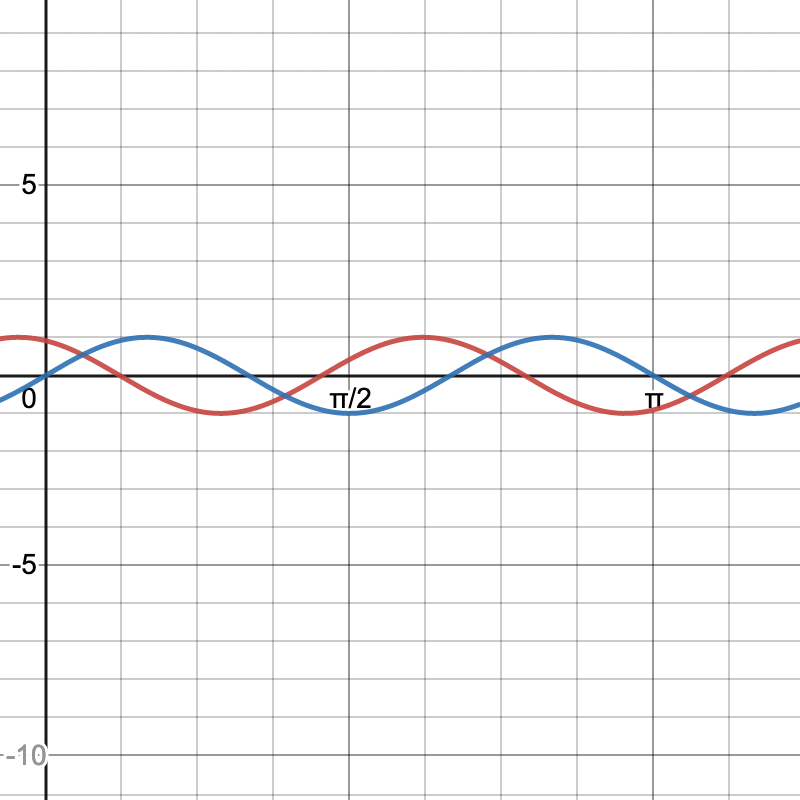
\includegraphics[width=0.5\textwidth]{figures/sine-wave-phase-shift.png}
	\caption{The phase shift in a sine wave}
	\label{fig:sine-wave-phase-shift}
\end{figure}


This type of sound modulation is done through a synthesizer's ``delay'' effect (sometimes known as ``echo'' effect). It is an effect which records an input signal, stores it, then plays it back after a defined time. Typically, the delayed audio is mixed with the live audio input creating an echo effect, where we first hear the original audio, followed by the delayed audio. The value of $D$ in Equation \ref{eq:sine-wave-equation} determines the shift of the wave, and thus also the sound. A positive value (such as $\frac{\pi}{2}$) will shift the sine wave to the left on the Cartesian plane, resulting in a sine wave which sounds early. The same applies to a negative $D$ value, in which a value such as $-\frac{\pi}{6}$ shifts the sine wave to the right, creating a sine wave which sounds ``late'' or delayed.

Other modules can be created through similar logic. To create legato and staccato, we either connect the waves of different frequencies together, or separate the waves to the point there is a clear distinction between the notes. Musically, these two concepts are total opposites; staccato is defined as the style of playing notes in a detached and separated manner, in which each note is clearly distinct from one another. It is typically indicated by a dot directly above or below the notehead, depending on if the stem of the note goes upwards (a dot is placed below the notehead), or goes downwards (a dot is placed above the notehead) \cite{Burkholder_Grout_Palisca_2014}. An example of staccato is in Figure \ref{fig:bartok-dance-five-b-section}, in which there are dots clearly above and below some of the notes, and the location of the dot is dependent on whether the stems of the notes face upwards or downwards. Legato is the directive which defines notes to be played in a smooth and connected manner, with notes that are no longer clearly distinctive from one another, as each note will flow gracefully into the next.

\begin{figure}[h]
  \centering
  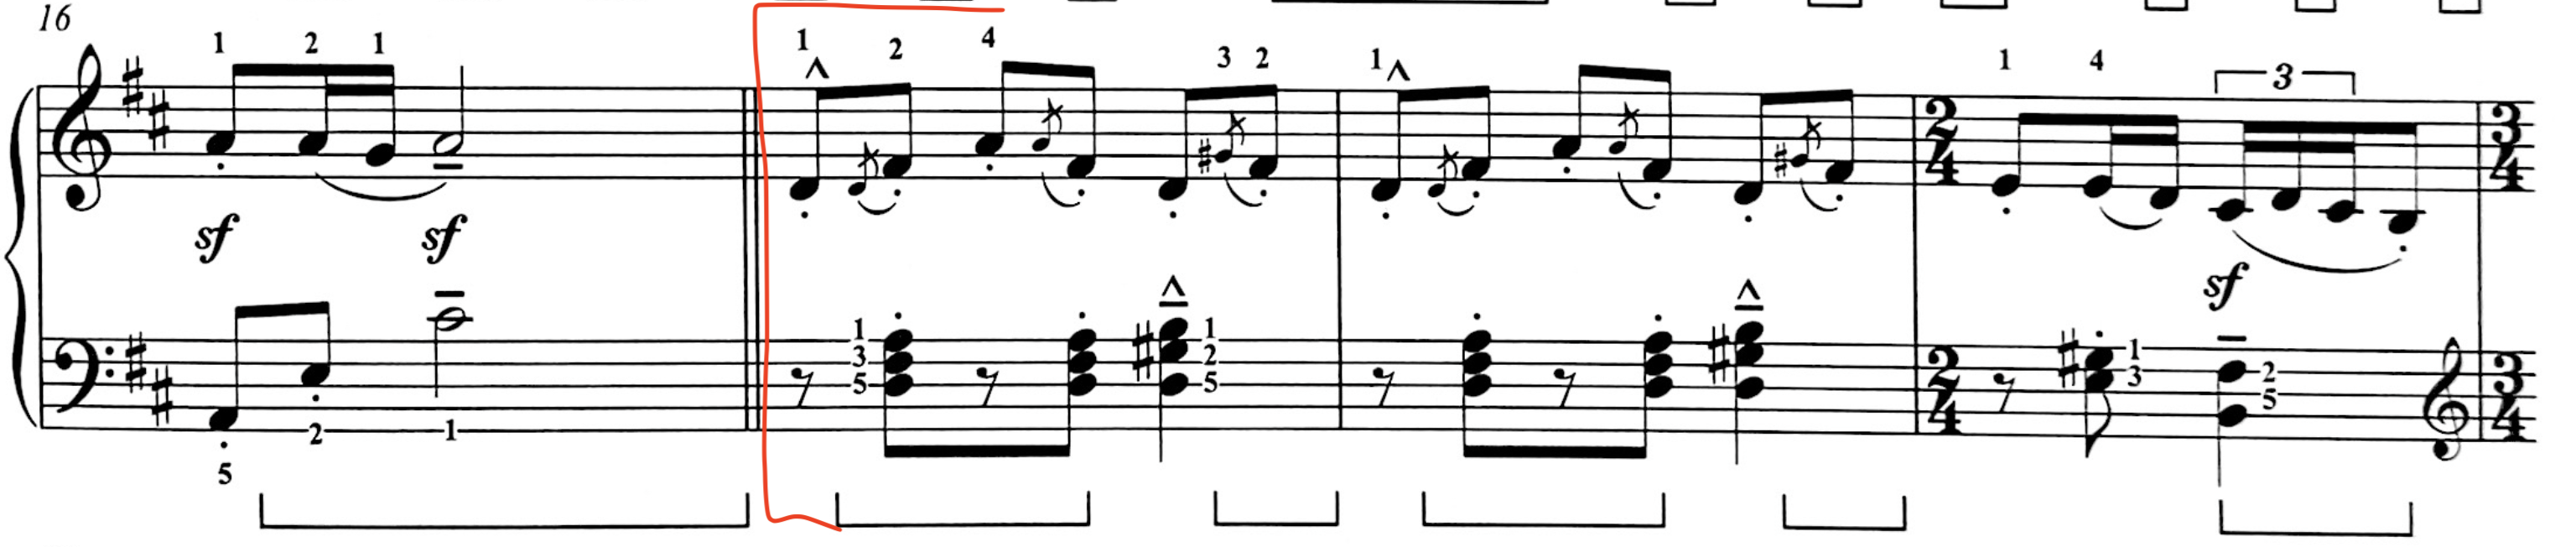
\includegraphics[width=\textwidth]{bartok-dance-five-b-section.jpg}
  \caption{Béla Bartók, Romanian Folk Dances, \textit{Poarga Românească}, mm. 16-19}
  \label{fig:bartok-dance-five-b-section}
\end{figure}

We will also create a module meant to layer two specific harmonics over a base frequency: the major third interval, and the perfect fifth interval, which together will form a major chord (refer to Appendix \ref{appendix:music-theory-terms}). Most chords are triadic in nature (that is, containing only three notes), with the interval of a major third or minor third between each of the three notes. The major third interval can be defined as the interval which spans four degrees of the diatonic scale in the Western twelve-semitone tuning system (refer to subsection \ref{subsection:how-midi}), or four semitones \cite{Nave_2017}.\footnote{The major third interval is also enharmonically equivalent to the diminished fourth interval. The enharmonic interval describes notes which sonically are the same, yet notated differently.} The minor third interval contains one fewer degrees than the major third interval, thus having only three degrees of the diatonic scale, and so only three semitones.

For instance, with a base frequency of the note $A$, the interval between $A$ and the note $C\musSharp{}$ is a major third interval. This interval spans the distance of four semitones. The distance between the note $A$ and the note $C$ is shorter than the distance between $A$ and $C\musSharp{}$, resulting in few semitones between the notes. This interval is the minor third interval, as the note $C$ is only three semitones away from the note $A$. A major interval will usually sound ``happier'' and brighter than a minor interval. The major third can give music a happy and playful tonality, while the minor third can result in music which sounds sad, dark, or spooky. It is important to understand the differences in the major and minor intervals--especially the major and minor thirds. These intervals can alter the timbre and quality of the sound (refer to Appendix \ref{appendix:music-theory-terms}) and the feeling of the music.

Songs which contain prominent examples of the major third interval include ``When the Saints Go Marching In,'' Ludwig van Beethoven's \textit{Fifth Symphony}, and the spiritual song and Christian hymn ``Swing Low, Sweet Chariot.'' In Figure \ref{fig:beethoven-fifth}, the notes must be read from the top of the sheet music down to the bottom--to understand the composite sound each instrument brings to the symphony--before being read from left-to-right. The first two measures of the symphony (before the blue line) show one major third interval, and the last two measures (after the blue line) show a different major third interval. These intervals do not sound as happy or bright as the major third interval may typically be, but the distinction between the major and minor third becomes easier to understand in comparison to a well-known piece which begins with the minor third interval: the English folk song ``Greensleeves.''

Songs which contain the minor third interval include ``Greensleeves'' (the first two notes), Christmas tune ``What Child Is This,'' and The Beatles' ``Hey, Jude.'' In Figure  \ref{fig:greensleeves}, the notes must also be read from top-down, before being read left-to-right. The first two notes of the piece (as bracketed in blue) demonstrate the minor third interval. In this piece, the notes played in the two clefs (the top: treble, the middle: alto, refer to Appendix \ref{appendix:music-theory-terms} for more details) are different pitches, but are still minor third intervals. For instance, the two notes played in the treble clef are $A$ and $C$. These notes create a sad, dark, and slightly ominous tonality to the song, a quality specific to the minor third interval. In comparison to the major third interval from Ludwig van Beethoven's \textit{Fifth Symphony}, it is clear that there is a difference in sound quality and tone between the two interval types. The major third interval, and thus the frequency difference between a base frequency and its corresponding major third interval, will sound brighter than the minor third interval. The frequency difference between a base frequency and its corresponding minor third interval results in a sad and dark sound quality. 

\begin{figure}[H]
  \centering
  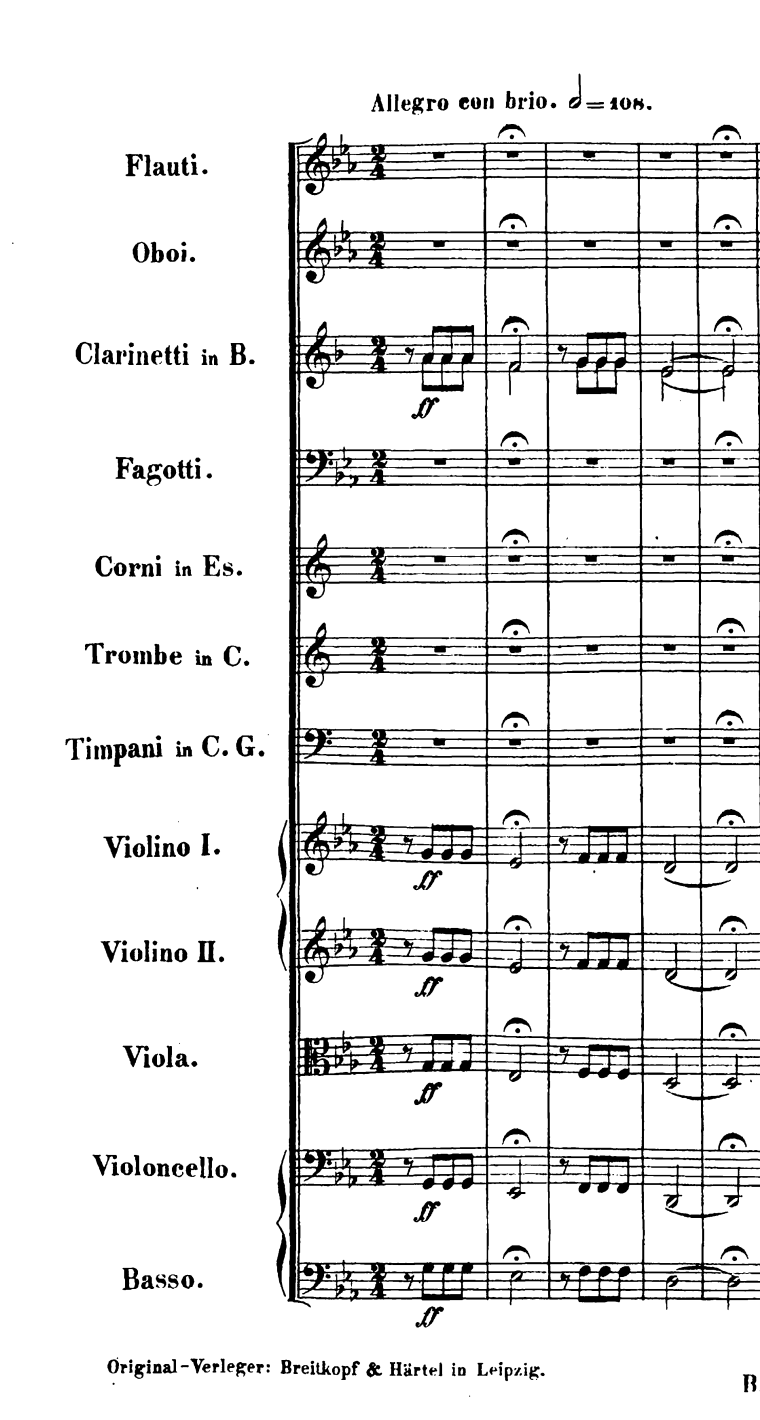
\includegraphics[width=0.5\textwidth]{beethoven-fifth.jpg}
  \caption{Ludwig van Beethoven, Symphony No. 5 in C Minor, \textit{Allegro con brio}, mm. 1-4}\cite{Beethoven_1862}
  \label{fig:beethoven-fifth}
\end{figure}

\begin{figure}[H]
  \centering
  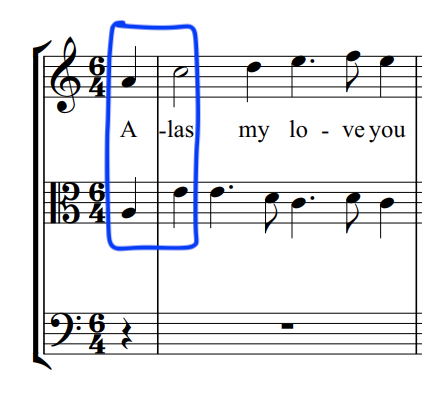
\includegraphics[width=0.4\textwidth]{greensleeves.jpg}
  \caption{``Greensleeves'', mm. 1}\cite{Kurtz_2010}
  \label{fig:greensleeves}
\end{figure}

The interval of the third is important to distinguish \textit{major} chords, and \textit{minor} chords, as major chords will have a root note (the tonic note, typically the first note played of a chord), major third interval, and another minor third interval (or perfect fifth interval above the tonic) stacked on top of one another, while a minor chord will have the tonic, minor third, and perfect fifth. Either multiple waveforms (of the specified major third and perfect fifth intervals) can be stacked to produce the major chord sound, or MIDI inputs (through the use of a MIDI device such as a MIDI keyboard) can trigger a major chord.

Another manipulation possible is to add the distortion alteration (as opposed to the specific distortion effect) to a sound is simply to add desired textures (additional layers, refer to Appendix \ref{appendix:music-theory-terms}). to a sound, through changing and deforming an audio signal's waveform. For many, a prime example is seen with the use of an electric guitar, as the pedals used with an electric guitar allow for added harmonics, and other changes made to the guitar's sound. One of the most used types of distortion is known as \textit{clipping}, in which the level of a signal (typically amplitude) goes beyond the maximum that a system is able to handle, leading to clipping, as the maximum of the waveforms gets abruptly cut off at the system's maximum. At its best form, distortion can be a gentle audio effect, which can add many types of sounds to a signal, including saturating the sound, and adding overdrive and \textit{fuzz}--two types of distortion effects--through adding \textit{gain} (defined as an increase in some type of value). With respect to distortion effects, \textit{gain} is referred to as \textit{transmission gain}, in which there is an increase in the power of a signal, expressed in \textit{decibels} (dB), usually done through an arbitrary combination of increasing the amplitude and frequency of a sound wave. This arbitrary combination of changes in frequency and amplitude can be done in all situations. The two most common, and most subtle, types of distortion are saturation and clipping. The result of these two types of clipping is ``soft clipping'' in which the peaks of the signal's waveform are softly rounded, and not abruptly cut off \cite{Tarr_2019}. The signal will be pushed only slightly over the 0 dB threshold. 

The concept of the 0 dB threshold is important for distortion effects, as it is a fundamental aspect to effectively create distortion within a modular synthesizer. Both digital and analog meters for volume, as in Figure \ref{fig:server-meter}, have ranges between negative infinity (or silence), up to 0 dB (the absolute loudest). In SuperCollider, this range will be between -80 and 0, as in Figure \ref{fig:server-meter}. These decibels are different than the standard decibels used to describe the loudness of everyday sounds. Standard decibels allow us to compare the relative loudness of sounds to each other; a jet taking off sounds at 140 dB, a firecracker is 140-165 dB, and a whisper may be 30 dB \cite{Hearing_Health_Foundation}. These decibels act as a unit measurement for sound, and the National Institute of Occupational Safety (NIOSH) \cite{Hearing_Health_Foundation} states that while exposure to noise at 85 decibels or above  will cause hearing loss, the exposure dangers for higher levels become exponentially more damaging. While at a noise level of 70 dB would take over 24 hours to cause hearing damage, sound at a level of 115 dB would cause hearing damage at only 28 seconds. The 115 dB volume of a rock concert and symphonic orchestra concert is much more noticeable, especially when comparing to the volume of listening to music on personal devices at maximum volume (105 dB).

The type of decibels used for music production are ``Decibels Full Scale'' (dBFS) when discussing digital music, or ``Sound Pressure Level'' (dB SPL) in the real world. This is the measurement of decibels as it pertains to the levels in an audio recording. Unlike the scale for dB, in which 0 dB is absolute silence, and higher numbers indicate a louder perceived volume, the scale for dBFS is reversed. With the dBFS scale, 0 dB is the maximum level of audio a system can process before it ``clips'' the signal. The lowest detectable level of sound in the system, the ``noise floor,''  can be as low as -150 dB, but is typically between -80 dB and -90 dB. In general, the common range for volume lies between -10 and -18 dB.
%, leaving 10 dB as headroom when combining all audio signals into one master track.

\begin{figure}[ht]
  \centering
  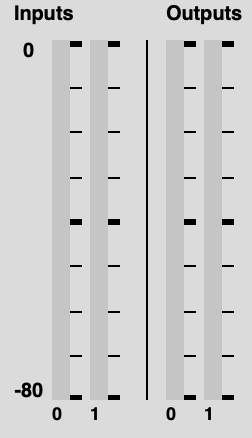
\includegraphics[width=0.2\textwidth]{server-meter.jpg}
  \caption{The server meter in SuperCollider}
  \label{fig:server-meter}
\end{figure}

So, keeping the noise level somewhere between -80 dB and -10 dB will help in introducing distortion to pure sound waveforms. If a signal is ``softly clipped'' (boosted slightly over the 0 dB threshold), the output sound may contain subtle harmonics (other frequencies overlaid on top of the original frequency) or other overtones. 

Overdrive, and fuzz--as previously mentioned--are two common types of distortion. In addition, the distortion effect itself (different from the class of sound alterations known as distortion), is another type of distortion. These three types of distortion effects tend to be synonymous with electric guitar rigs, pedals, and other similar hardware. Overdrive tends to be the most subtle of the three, with higher gain levels. Distortion and fuzz are more intense, with distortion allowing for large amounts of sustain, harmonics, and a mostly altered sound from the original input, noticeable in heavy rock music and guitar solos. Fuzz is similar to distortion in gain level, but will produce a sound similar to that of a square wave. Distortion using the fuzz effect produces a traditional synth-like effect, with digital artifacts, or overly processed sounds.
